\subsection{Atomic goals}
Besides Composite goals, we also have Atomic goals. You can compare Atomic 
goals with leaf nodes of a tree structure. Atomic goals are the actual actions
 that an entity needs to do. As shown in \cref{fig:atomicgoal-inherit}, an atomic 
 goal has no subgoals. Calling the AtomicGoal::add\_subgoal() method results in an 
 exception.
 
 \begin{figure}[!htb]
    \centering
    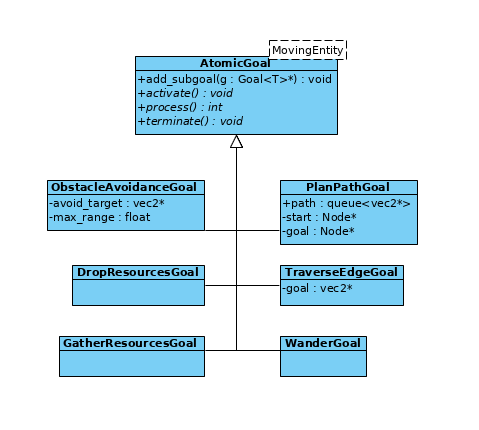
\includegraphics{res/AtomicGoal-Inherit.jpg}
    \caption{AtomicGoal Inheritance.}\label{fig:atomicgoal-inherit}
\end{figure}

\subsubsection{Wander}
The wandering goal is another goal that never gets removed, just like the 
think goal. An entity always needs to wander around if it has absolutely 
nothing to do. The only thing this goal does is activate the wander steering 
behaviour (\cref{sec:wander}).

\subsubsection{Obstacle Avoidance}
The obstacle avoidance goal activates the obstacle avoidance steering 
behaviour. When this goal is activated, it adds the steering behaviour to the 
entity's behaviours. Once the distance to the target that it needs to avoid 
is big enough, the goal is completed and the steering behaviour also gets 
removed from the entity.

\subsubsection{Drop Resources}
\label{sec:dropresources}
Once an entity has gathered enough resources, it needs to drop them at a 
warehouse/depot. This goal simply removes the resources the entity gathered and adds them to the resources of the player. When it dropped all of it's resources at the warehouse, the goal is completed.

\subsubsection{Gather Resource}
\label{sec:gatherresource}
This goal calls the Gather() method from a resource entity. This method extracts resources from the resource entity and adds it to the entity that is gathering the resource. Once the resource entity has been depleted or the maximum carrying capacity of the gathering entity has been reached this goal will be completed.

\subsubsection{Plan Path}
\label{sec:planpath}
The plan path goal plans a path using the A* algorithm, using the Manhattan 
heuristic (\cref{sec:pathplanning}). Once the path has been generated, it gets set as the active path 
for the given entity. This is the only task it needs to complete before 
getting removed from the containing goal.

\subsubsection{Traverse Edge}
\label{sec:traverseedge}
This goal uses the Seek behaviour explained in \cref{sec:seek-behaviour}. Once 
this class gets instantiated it adds an instance of SeekStrategy to the 
entity's behaviour. The only thing it needs to do while processing, is 
to check whether the entity has this behaviour, and if so if it's close 
enough to the next node on the graph. If it's close enough, the goal has been 
completed.

